\documentclass[tikz,border=10pt]{standalone}
\begin{document}
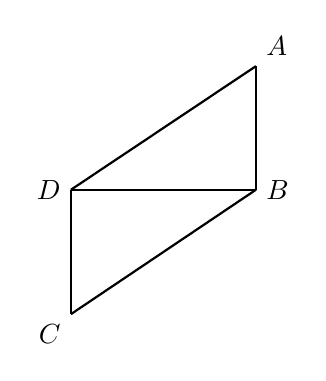
\begin{tikzpicture}[line width=0.8pt]
  \coordinate (A) at (2.35,1.57);
  \coordinate (B) at (2.35,0);
  \coordinate (C) at (0,-1.58);
  \coordinate (D) at (0,0);

  \draw (A) -- (D);
  \draw (D) -- (B);
  \draw (A) -- (B);
  \draw (D) -- (C);
  \draw (C) -- (B);

  \node[above right] at (A) {$A$};
  \node[right] at (B) {$B$};
  \node[left] at (D) {$D$};
  \node[below left] at (C) {$C$};
\end{tikzpicture}
\end{document}
